%%%%%%%%%%%%%%%%%%%%%%%%%%%%%%%%%%%%%%
%%%%%%%%%%%%%%%%%%%%%%%%%%%%%%%%%%%%%%
% Do not edit the TeX file your work
% will be overwritten.  Edit the RnW
% file instead.
%%%%%%%%%%%%%%%%%%%%%%%%%%%%%%%%%%%%%%
%%%%%%%%%%%%%%%%%%%%%%%%%%%%%%%%%%%%%%



Here are results, and a figure. See \figref{example_genes}.
%

\begin{knitrout}
\definecolor{shadecolor}{rgb}{0.969, 0.969, 0.969}\color{fgcolor}\begin{kframe}


{\ttfamily\noindent\bfseries\color{errorcolor}{\#\# Error in py\_call\_impl(callable, dots\$args, dots\$keywords): FileNotFoundError: [Errno 2] No such file or directory: './R\_scripts/mice/data/example\_genes.npz'\\\#\# \\\#\# Detailed traceback: \\\#\#\ \  File "{}/home/rgiordan/.local/lib/python3.8/site-packages/numpy/lib/npyio.py"{}, line 416, in load\\\#\#\ \ \ \  fid = stack.enter\_context(open(os\_fspath(file), "{}rb"{}))}}\end{kframe}
\end{knitrout}
%






\begin{knitrout}
\definecolor{shadecolor}{rgb}{0.969, 0.969, 0.969}\color{fgcolor}\begin{kframe}


{\ttfamily\noindent\bfseries\color{errorcolor}{\#\# Error in py\_call\_impl(callable, dots\$args, dots\$keywords): FileNotFoundError: [Errno 2] No such file or directory: './R\_scripts/mice/data/fitted\_centroids.npz'\\\#\# \\\#\# Detailed traceback: \\\#\#\ \  File "{}/home/rgiordan/.local/lib/python3.8/site-packages/numpy/lib/npyio.py"{}, line 416, in load\\\#\#\ \ \ \  fid = stack.enter\_context(open(os\_fspath(file), "{}rb"{}))}}\end{kframe}
\end{knitrout}







\begin{knitrout}
\definecolor{shadecolor}{rgb}{0.969, 0.969, 0.969}\color{fgcolor}\begin{kframe}


{\ttfamily\noindent\bfseries\color{errorcolor}{\#\# Error in py\_call\_impl(callable, dots\$args, dots\$keywords): FileNotFoundError: [Errno 2] No such file or directory: './R\_scripts/mice/data/coclustering\_alpha1.0.npz'\\\#\# \\\#\# Detailed traceback: \\\#\#\ \  File "{}/home/rgiordan/.local/lib/python3.8/site-packages/numpy/lib/npyio.py"{}, line 416, in load\\\#\#\ \ \ \  fid = stack.enter\_context(open(os\_fspath(file), "{}rb"{}))}}

{\ttfamily\noindent\bfseries\color{errorcolor}{\#\# Error in as.data.frame(file[[key]]): object 'alpha1\_coclust\_file' not found}}

{\ttfamily\noindent\bfseries\color{errorcolor}{\#\# Error in plot\_coclustering(coclust\_init): object 'coclust\_init' not found}}\end{kframe}\begin{figure}[!h]

{\centering 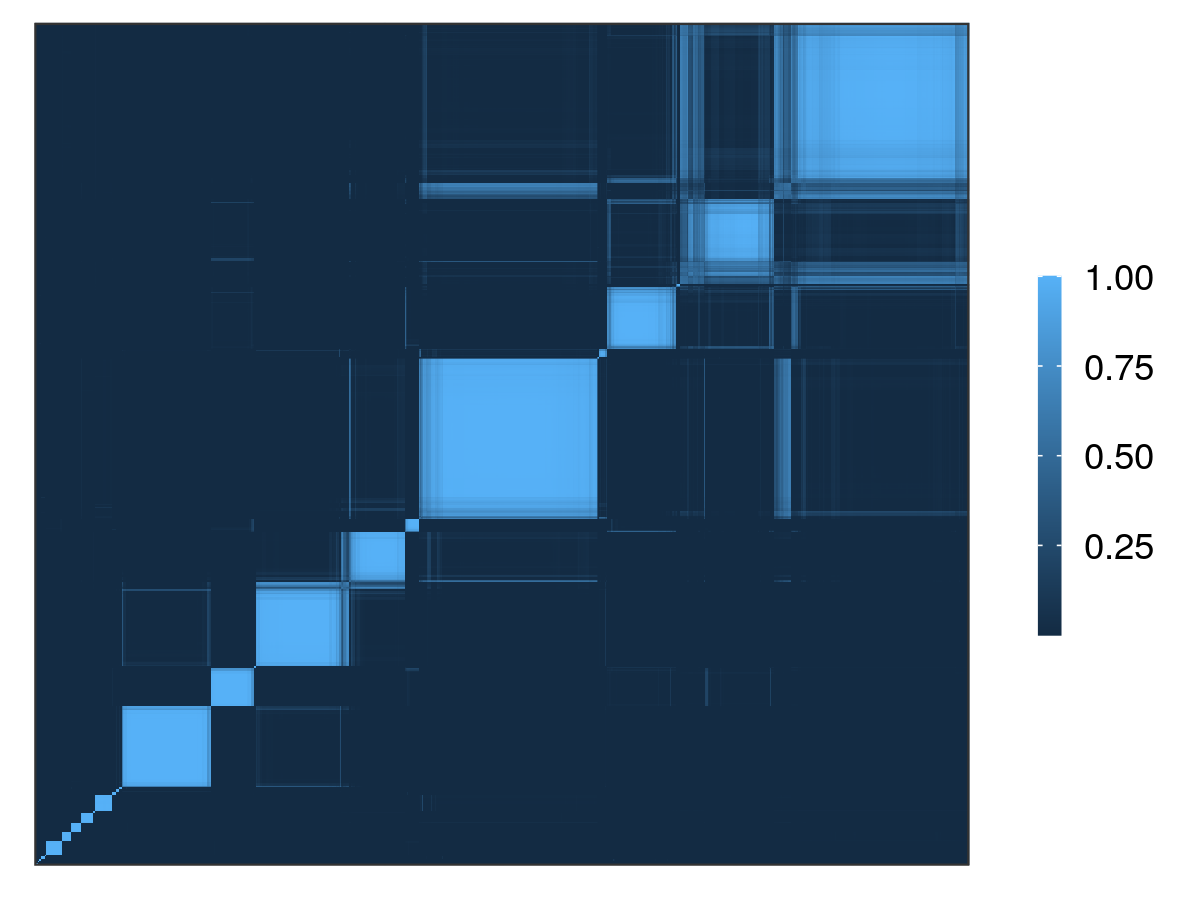
\includegraphics[width=0.98\linewidth,height=0.666\linewidth]{./R_scripts/mice/figures_tmp/init_coclustering} 

}

\caption[The inferred co-clustering matrix at alpha = 3]{The inferred co-clustering matrix at alpha = 3. }\label{fig:gene_initial_coclustering}
\end{figure}


\end{knitrout}










\begin{knitrout}
\definecolor{shadecolor}{rgb}{0.969, 0.969, 0.969}\color{fgcolor}\begin{kframe}


{\ttfamily\noindent\bfseries\color{errorcolor}{\#\# Error in py\_call\_impl(callable, dots\$args, dots\$keywords): FileNotFoundError: [Errno 2] No such file or directory: './R\_scripts/mice/data/coclustering\_alpha1.0.npz'\\\#\# \\\#\# Detailed traceback: \\\#\#\ \  File "{}/home/rgiordan/.local/lib/python3.8/site-packages/numpy/lib/npyio.py"{}, line 416, in load\\\#\#\ \ \ \  fid = stack.enter\_context(open(os\_fspath(file), "{}rb"{}))}}\end{kframe}\begin{figure}[!h]

{\centering 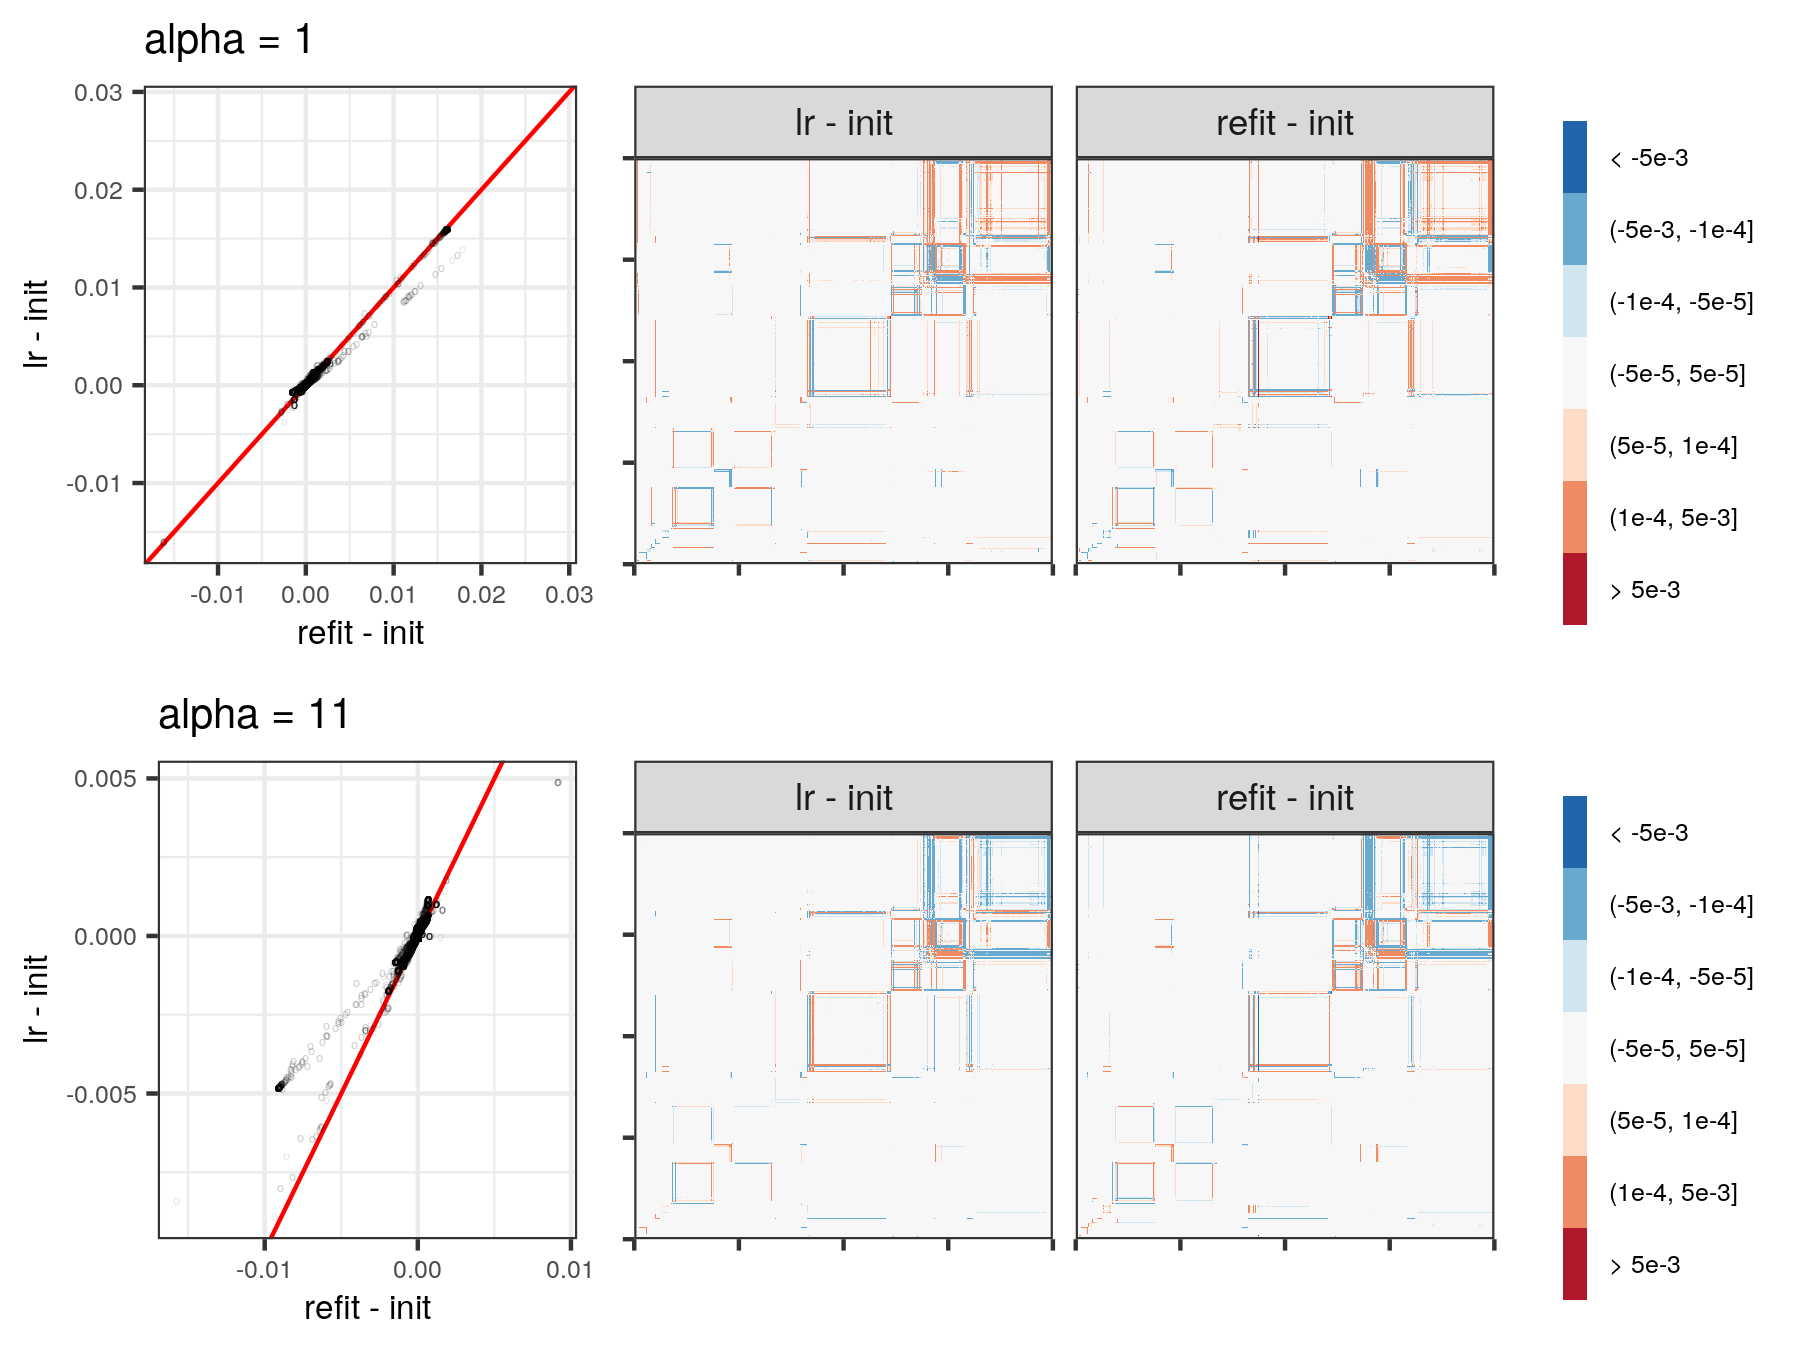
\includegraphics[width=0.98\linewidth,height=0.588\linewidth]{./R_scripts/mice/figures_tmp/alpha_coclust_sensitivity} 

}

\caption[Changes in the co-clustering matrix at alpha = 1 (top row)
     and alpha = 11 (bottom row),
     relative to the co-clustering matrix at alpha = 3.
     The left column plots differences predicted by the
     linear approximation against differences from a model refit.
     Each point represents an entry of the co-clusteirng matrix.
     The middle and right columns display
     changes in the co-clustering matrix as obtained by the
     linear approximation and the model refit, respectively]{Changes in the co-clustering matrix at alpha = 1 (top row)
     and alpha = 11 (bottom row),
     relative to the co-clustering matrix at alpha = 3.
     The left column plots differences predicted by the
     linear approximation against differences from a model refit.
     Each point represents an entry of the co-clusteirng matrix.
     The middle and right columns display
     changes in the co-clustering matrix as obtained by the
     linear approximation and the model refit, respectively.}\label{fig:gene_alpha_coclustering}
\end{figure}


\end{knitrout}





\begin{knitrout}
\definecolor{shadecolor}{rgb}{0.969, 0.969, 0.969}\color{fgcolor}\begin{kframe}


{\ttfamily\noindent\bfseries\color{errorcolor}{\#\# Error in py\_call\_impl(callable, dots\$args, dots\$keywords): FileNotFoundError: [Errno 2] No such file or directory: './R\_scripts/mice/data/coclustering\_worstcase.npz'\\\#\# \\\#\# Detailed traceback: \\\#\#\ \  File "{}/home/rgiordan/.local/lib/python3.8/site-packages/numpy/lib/npyio.py"{}, line 416, in load\\\#\#\ \ \ \  fid = stack.enter\_context(open(os\_fspath(file), "{}rb"{}))}}\end{kframe}
\end{knitrout}





\begin{knitrout}
\definecolor{shadecolor}{rgb}{0.969, 0.969, 0.969}\color{fgcolor}\begin{kframe}


{\ttfamily\noindent\bfseries\color{errorcolor}{\#\# Error in py\_call\_impl(callable, dots\$args, dots\$keywords): FileNotFoundError: [Errno 2] No such file or directory: './R\_scripts/mice/data/functional\_coclustering\_gauss\_pert1.npz'\\\#\# \\\#\# Detailed traceback: \\\#\#\ \  File "{}/home/rgiordan/.local/lib/python3.8/site-packages/numpy/lib/npyio.py"{}, line 416, in load\\\#\#\ \ \ \  fid = stack.enter\_context(open(os\_fspath(file), "{}rb"{}))}}\end{kframe}\begin{figure}[!h]

{\centering 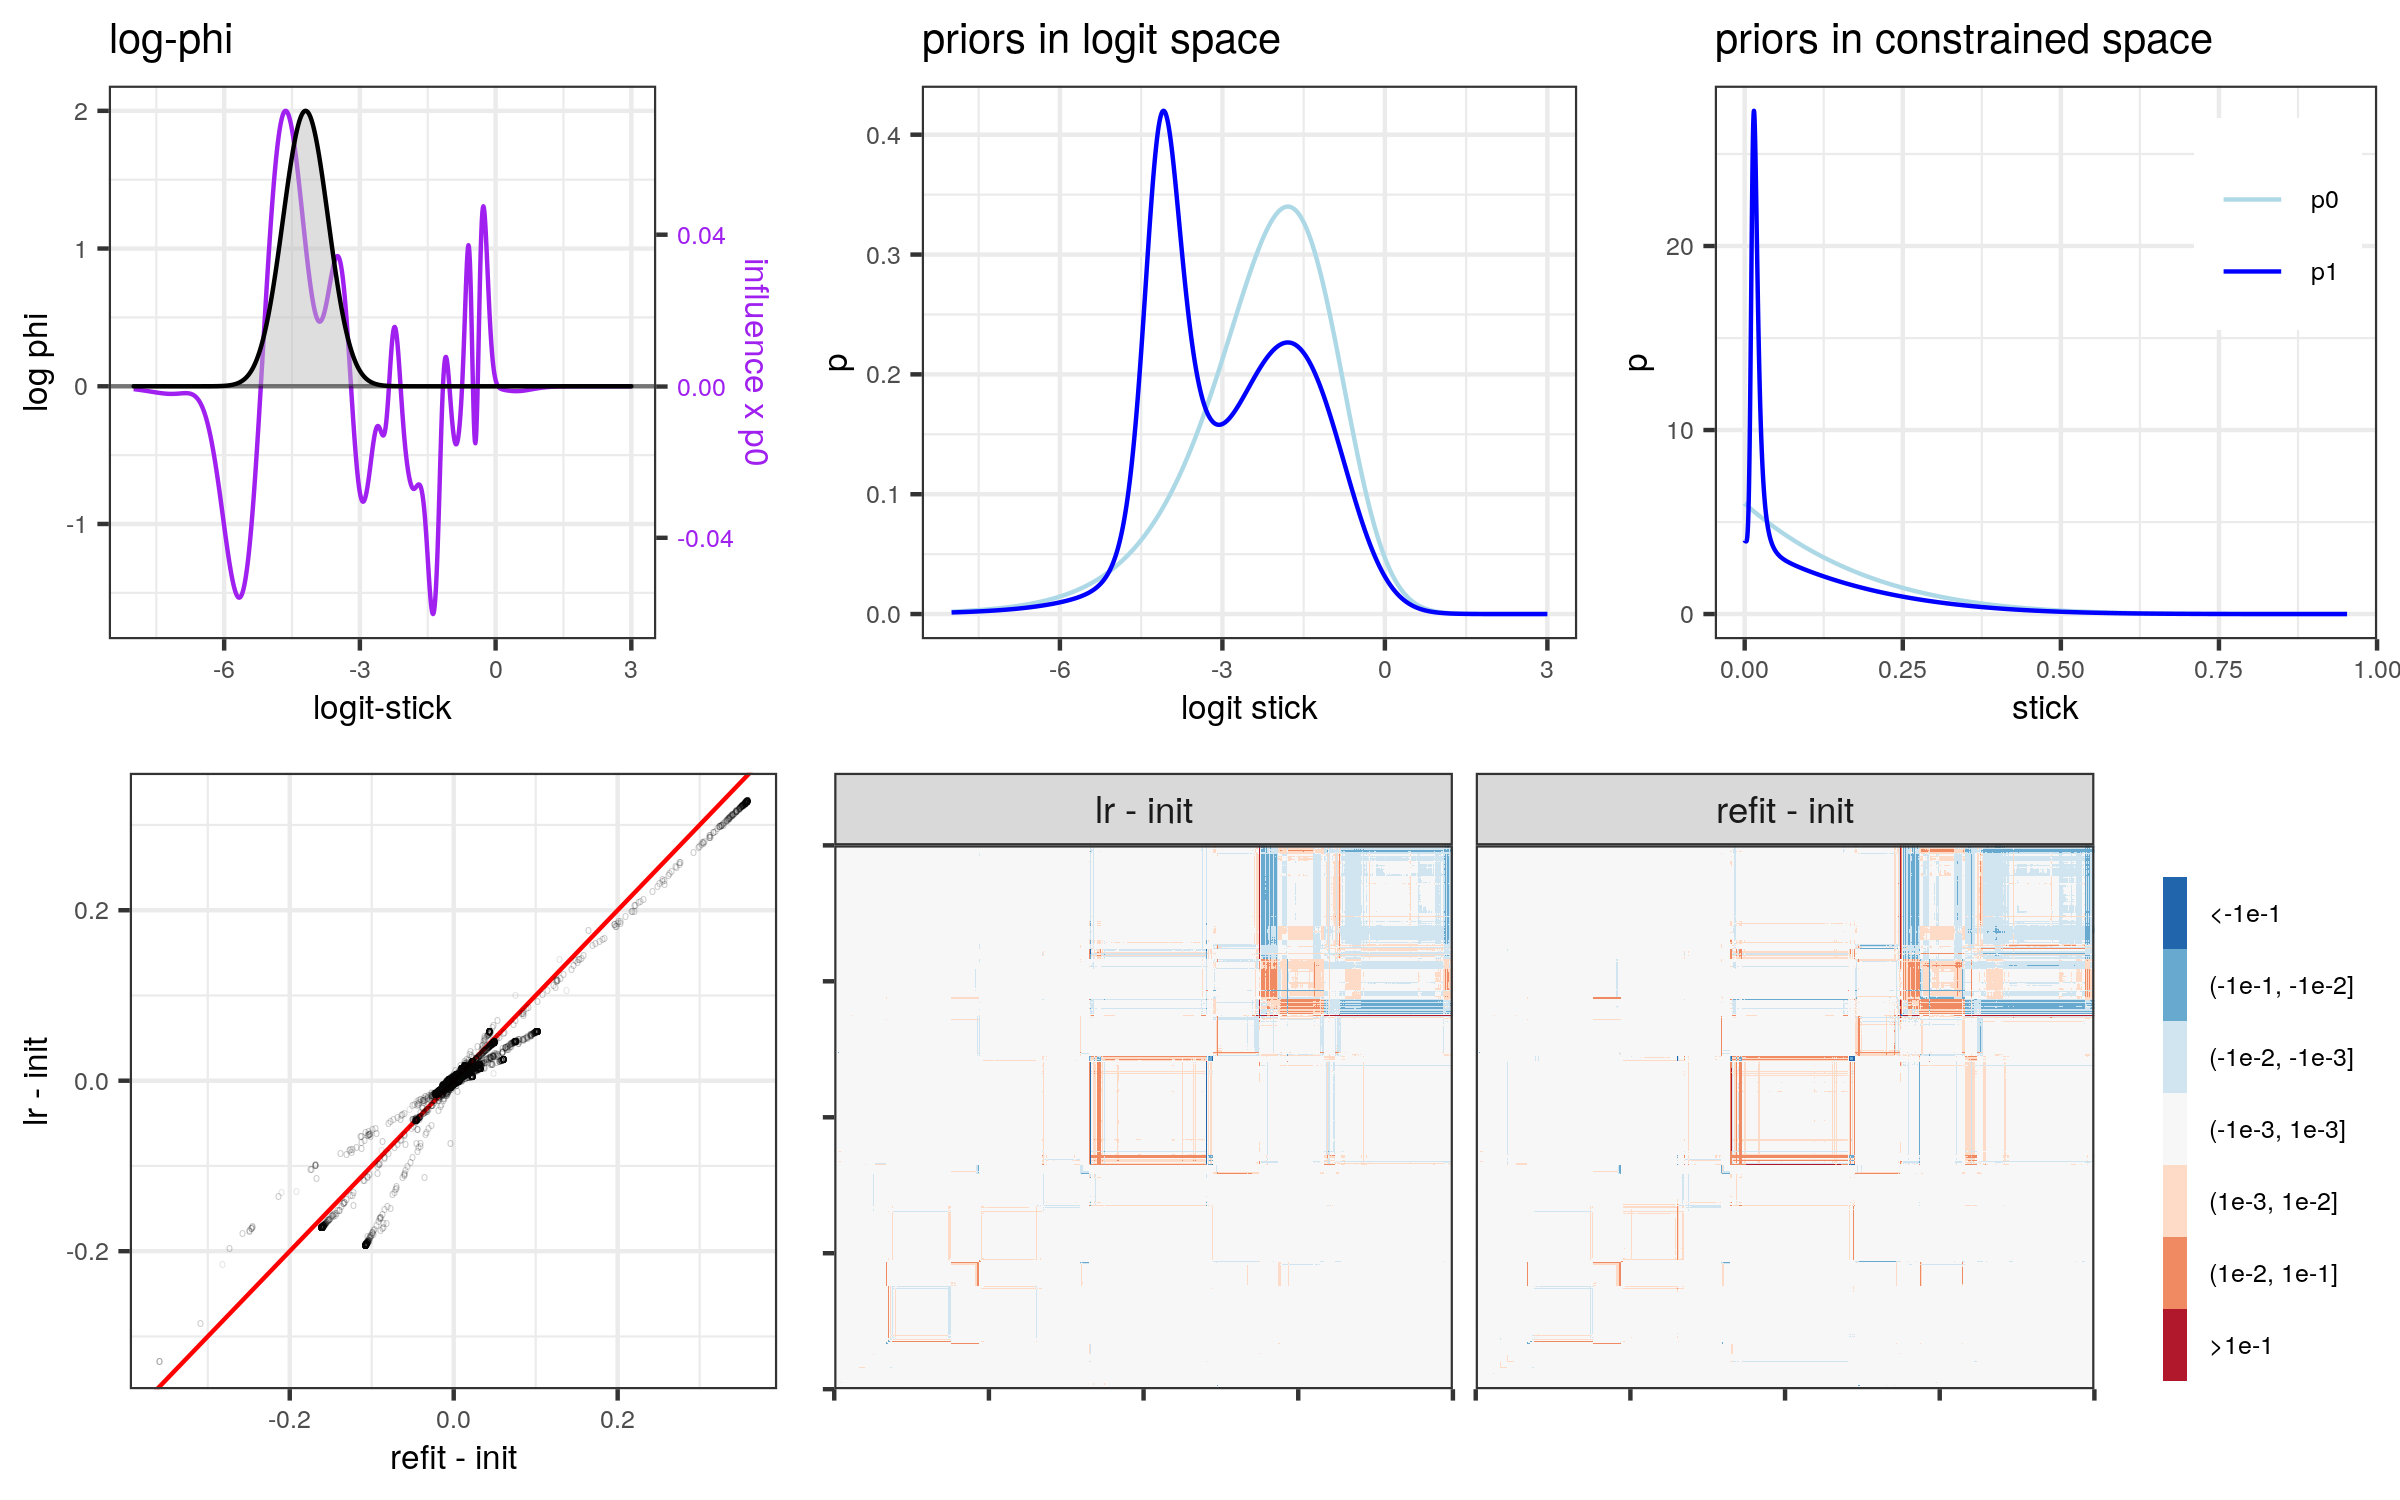
\includegraphics[width=0.98\linewidth,height=0.627\linewidth]{./R_scripts/mice/figures_tmp/fpert_coclust_sensitivity} 

}

\caption[Effect on the co-clustering matrix after a functional perturbation.
     log-phi (top left, in grey) is set to a Gaussian p.d.f]{Effect on the co-clustering matrix after a functional perturbation.
     log-phi (top left, in grey) is set to a Gaussian p.d.f. centered at mu = -4.2, and scaled to have L-infinity norm equal to two.
    The chosen log-phi roughly corresponds to a positive bump in the influence function of $g_{ev}$.}\label{fig:gene_fpert_coclustering}
\end{figure}


\end{knitrout}
